\chapter{Sprint0: Analyse et conception globales }


\section{Introduction}
Ce chapitre sera dédié à l'analyse et à la spécification des besoins. 
En premier lieu, nous identifierons les acteurs principaux du projet. En second lieu, nous définirons les différents besoins fonctionnels et non fonctionnels de notre application. 
Par la suite, nous présenterons une étude conceptuelle globale. Enfin, nous clôturons par définir l'architecture utilisée.


\section{Identification des acteurs}
Un acteur présente une personne, une entité ou un système  agissant d'une façon directe sur l'application.\\
Les différents acteurs modélisant notre système sont :
\begin{itemize}
	\item  \textit{Utilisateur} : un employé de l'entreprise qui peut gérer son profil, consulter ses instances, gérer les planifications, etc.
	\item  \textit{Chef de projet}  est un membre de la société, qui peut en plus des fonctionnalités récemment citées créer de nouvelle instance cloud, gérer des membres de son projet, etc.
	\item  \textit{Administrateur}  directeur technique de l'entreprise et la personne la plus privilégiée, il possède le droit de manipuler toutes les fonctionnalités offertes par notre application.
\end{itemize}
L'ensemble de ces acteurs sont liées par une relation d'héritage. 
\section{Identification des besoins}
Dans cette section, nous allons développer les besoins fonctionnels et non fonctionnels de l'entreprise d'accueil.
\subsection{Besoins fonctionnels}
Les besoins fonctionnels expriment les principales fonctionnalités de l'application sans se
préoccuper de la façon de l'implémentation.\\
Une étude détaillée de système nous a permis de dégager les principaux exigences fonctionnelles
des différents acteurs de notre application.
\begin{itemize}
	\item Authentification et gestion de mot de passe.
	\item Consultation et modification du profil.
	\item Gestion des projets notamment création, suppression et modification.
	\item Gestion des utilisateurs qui contient le volet de consultation et de suppression.
		\item Gestion des planifications notamment création et suppression.
	\item Affectation/ retrait d'un projet à un utilisateur.
	\item Affectation/retrait d'un planning des instances de machines virtuelles.
	\item Manipulation des instances de machine virtuelle. Un utilisateur peut consulter, activer, arrêter 
	une instance.
	\item Attribution des droits d'accès différents selon l'utilisateur.
	\item Gestion des machines virtuelles.
	\item Gestion des instances de machine virtuelle qui contient le volet de création et de suppression réalisée que par le chef de projet et l'administrateur.
\end{itemize}


\subsection{Besoins non fonctionnels}
Pour garantir un bon fonctionnement de l'application, cette dernière doit assurer les besoins non fonctionnels présentés ci-dessous.
\begin{itemize}
	\item Ergonomie : Les interfaces doivent être conviviales, ergonomiques et facile à exploiter par l'utilisateur.
	\item Fiabilité : L'application doit fournir des résultats correctes.
	\item Sécurité : L'accès à l'application ainsi qu'aux données doit être sécurisé. D'une part par
	la gestion des autorisations aux différents modules de l'application grâces aux privilèges
	gérés par le module d'administration et d'une autre part par l'intégration d'un module
	d'authentification basée sur l'échange de jetons  entre le serveur et le client.
	\item Extensibilité : Le système doit être extensible et permet de s'intégrer facilement sur le réseau existant  de l'entreprise. Il doit aussi supporter l'intégration d'autres fonctionnalités
	\item  Maintenabilité : La maintenabilité et l'évolutivité sont des priorités. Le code sera lisible,
	commenté, divisé en fonction des pages (des interfaces) et en fonction des tâches abordées.

\end{itemize}
\section{Étude conceptuelle}

Nous allons exposer dans cette section le diagramme de cas d'utilisation et de classe globales modélisant notre projet.

\subsection {Diagramme de cas d'utilisation global }
Dans cette partie, nous présentons le diagramme de cas d'utilisation global qui modélise
l'interaction entre le système informatique à développer et les acteurs interagissant avec le système.
Également, il permet de recenser  les besoins des utilisateurs et les fonctionnalités du système.
\newpage
\begin{figure}[H]
	\centering
	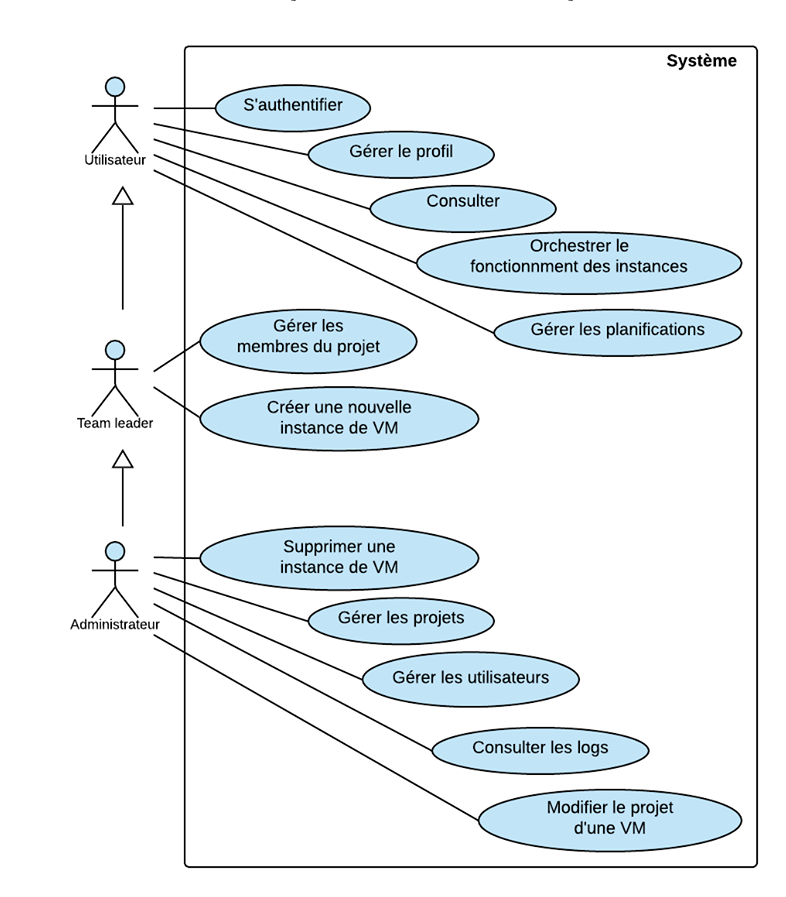
\includegraphics[scale=0.5]{DCUglobal.png}
	\caption{Diagramme de cas d'utilisation global}
	\label{Diagramme de cas d'utilisation global}
\end{figure}
 La figure 2.1 ci-dessus représente le diagramme de cas d'utilisation global de notre
projet où on y trouve les acteurs principaux et leurs rôles.\\ Ce diagramme décrit de manière globale les différentes fonctionnalités de chaque acteur. 
En effet, tout utilisateur est apte à s'authentifier, gérer son profil, consulter les projets,  gérer les planifications de fonctionnement des machines virtuelles et orchestrer leurs fonctionnements.
Notre deuxième acteur est un Team leader qui est utilisateur privilégié par la gestion des membres du projet et la création des machines virtuelles.
De plus que les fonctionnalités de Team leader et d'utilisateur, l'administrateur assure la gestion des utilisateurs et la consultation des logs.
\section{Étude conceptuelle globale}
\subsection{Diagramme de classe global}
Le diagramme de classe  est considéré parmi les diagrammes les plus importants dans la modélisation  de l'UML(Unified Modeling Language), comme présenté dans la figure 2.2, il permet de décrire la structure statique d'un système en présentant ses différents classes, attributs, méthodes et relations entre ses objets. 

\begin{figure}[H]
	\centering

	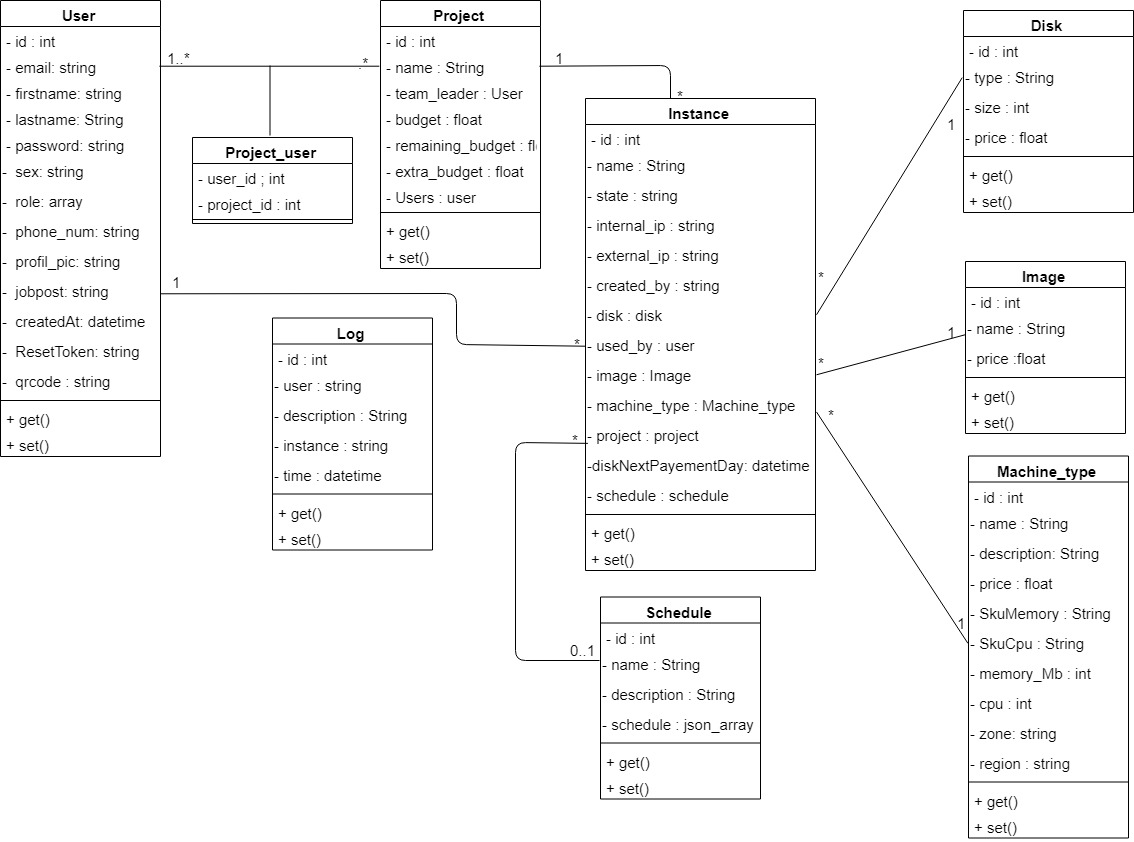
\includegraphics[ height=16cm, width=16cm]{diagdeclass.jpg}
	\caption{Diagramme de classe global}
	\label{Diagramme de classe global}
\end{figure}

\section{Spécifités techniques}
\subsection{Backlog produit}
Le Backlog est un artéfact très important dans Scrum. C'est l'ensemble des
caractéristiques fonctionnelles ou techniques qui constituent le produit souhaité.
Le tableau 2.1 résume le backlog produit de notre application où chaque user story est
caractérisé par un identifiant, un nom et une estimation.

% Please add the following required packages to your document preamble:
% \usepackage{multirow}
\begin{table}[H]
	\begin{tabular}{|l|l|l|l|}
		\hline
		\textbf{ID}        & \textbf{Tâches}                             & \textbf{User Story}                                                                                                                                       & \textbf{Esti.} \\ \hline
		\multirow{5}{*}{1} & \multirow{5}{*}{Gestion des comptes}        & \begin{tabular}[c]{@{}l@{}}1.1 En tant que utilisateur, je souhaite \\ m'inscrire à l'application.\end{tabular}                                           & 3              \\ \cline{3-4} 
		&                                             & \begin{tabular}[c]{@{}l@{}}1.2 En tant que utilisateur, je souhaite\\ m'authentifier à l'application.\end{tabular}                                        & 5              \\ \cline{3-4} 
		&                                             & \begin{tabular}[c]{@{}l@{}}1.3 En tant que utilisateur je souhaite \\ recevoir un mail de réinitialisation du mot\\ de passe en cas d'oubli.\end{tabular} & 5              \\ \cline{3-4} 
		&                                             & \begin{tabular}[c]{@{}l@{}}1.4 En tant que utilisateur, je souhaite\\ consulter mon profil.\end{tabular}                                                  & 3              \\ \cline{3-4} 
		&                                             & \begin{tabular}[c]{@{}l@{}}1.5 En tant que utilisateur, je souhaite \\ mettre à jour mes données personnelles.\end{tabular}                               & 3              \\ \hline
		\multirow{4}{*}{2} & \multirow{4}{*}{Gestion des utilisateurs}   & \begin{tabular}[c]{@{}l@{}}2.1 En tant que administrateur, je souhaite\\ consulter la liste des utilisateurs de \\ l'application\end{tabular}             & 2              \\ \cline{3-4} 
		&                                             & \begin{tabular}[c]{@{}l@{}}2.2 En tant que administrateur, je souhaite\\ supprimer un utilisateur.\end{tabular}                                           & 2              \\ \cline{3-4} 
		&                                             & \begin{tabular}[c]{@{}l@{}}2.3 En tant que administrateur, je souhaite\\ affecter un projet à un utilisateur.\end{tabular}                                & 3              \\ \cline{3-4} 
		&                                             & \begin{tabular}[c]{@{}l@{}}2.4 En tant que administrateur, je souhaite\\ retirer un projet d'un utilisateur.\end{tabular}                                 & 3              \\ \hline
		\multirow{6}{*}{3} & \multirow{6}{*}{Management des projets}     & \begin{tabular}[c]{@{}l@{}}3.1 En tant que Team leader, je souhaite\\ consulter mes projets.\end{tabular}                                                 & 2              \\ \cline{3-4} 
		&                                             & \begin{tabular}[c]{@{}l@{}}3.2 En tant que administrateur, je souhaite\\ supprimer un projet.\end{tabular}                                                & 2              \\ \cline{3-4} 
		&                                             & \begin{tabular}[c]{@{}l@{}}3.3 En tant que administrateur, je souhaite \\ créer un projet.\end{tabular}                                                   & 2              \\ \cline{3-4} 
		&                                             & \begin{tabular}[c]{@{}l@{}}3.4 En tant que administrateur, je souhaite\\ modifier un projet.\end{tabular}                                                 & 2              \\ \cline{3-4} 
		&                                             & \begin{tabular}[c]{@{}l@{}}3.5 En tant que Team leader, je souhaite \\ ajouter un membre à mon projet.\end{tabular}                                       & 3              \\ \cline{3-4} 
		&                                             & \begin{tabular}[c]{@{}l@{}}3.6 En tant que Team leader, je souhaite \\ retirer un membre de mon projet.\end{tabular}                                      & 3              \\ \hline
		\multirow{5}{*}{4} & \multirow{5}{*}{Management des VMs}         & \begin{tabular}[c]{@{}l@{}}4.1 En tant que utilisateur je souhaite \\ consulter la liste des VMs.\end{tabular}                                            & 5              \\ \cline{3-4} 
		&                                             & \begin{tabular}[c]{@{}l@{}}4.2 En tant que utilisateur je souhaite \\ orchestrer le fonctionnement des VMs.\end{tabular}                                  & 5              \\ \cline{3-4} 
		&                                             & \begin{tabular}[c]{@{}l@{}}4.3 En tant que Team leader je souhaite créer\\ de nouvelles instances de machine \\ virtuelle.\end{tabular}                   & 7              \\ \cline{3-4} 
		&                                             & \begin{tabular}[c]{@{}l@{}}4.4 En tant que administrateur, je souhaite\\ supprimer  une machine virtuelle.\end{tabular}                                   & 7              \\ \cline{3-4} 
		&                                             & \begin{tabular}[c]{@{}l@{}}4.5 En tant que administrateur, je souhaite\\ modifier le projet d'une machine virtuelle.\end{tabular}                         & 3              \\ \hline
		\end{tabular}
\end{table}

\begin{table}[H]
	\begin{tabular}{|l|l|l|l|}
		\hline
		\textbf{ID}        & \textbf{Tâches}                             & \textbf{User Story}                                                                                                                                       & \textbf{Esti.} \\ \hline
	\multirow{5}{*}{5} & \multirow{5}{*}{Gestion des planifications} & \begin{tabular}[c]{@{}l@{}}5.1 En tant que utilisateur, je souhaite \\ consulter la liste des plannings.\end{tabular}                                     & 2              \\ \cline{3-4} 
&                                             & \begin{tabular}[c]{@{}l@{}}5.2 En tant que utilisateur, je souhaite créer \\ un planning.\end{tabular}                                                    & 4              \\ \cline{3-4} 
&                                             & \begin{tabular}[c]{@{}l@{}}5.3 En tant que utilisateur,je souhaite \\ supprimer un planning.\end{tabular}                                                 & 3              \\ \cline{3-4} 
&                                             & \begin{tabular}[c]{@{}l@{}}5.4 En tant que utilisateur, je souhaite affecter\\ un planning à une VM.\end{tabular}                                         & 5              \\ \cline{3-4} 
&                                             & \begin{tabular}[c]{@{}l@{}}5.5 En tant que utilisateur, je souhaite retirer\\ un planning d'une VM.\end{tabular}                                          & 3              \\ \hline
6                  & Gestion des logs                            & \begin{tabular}[c]{@{}l@{}}6.1 En tant que utilisateur, je souhaite \\ consulter les activités des utilisateurs.\end{tabular}                             & 3              \\ \hline

	\end{tabular}
\caption{Backlog produit}
\label{Backlog produit}
\end{table}

\subsection{Planification du projet}
La planification de notre projet est résumée par  la figure 2.3
\begin{figure}[h]
	\centering
	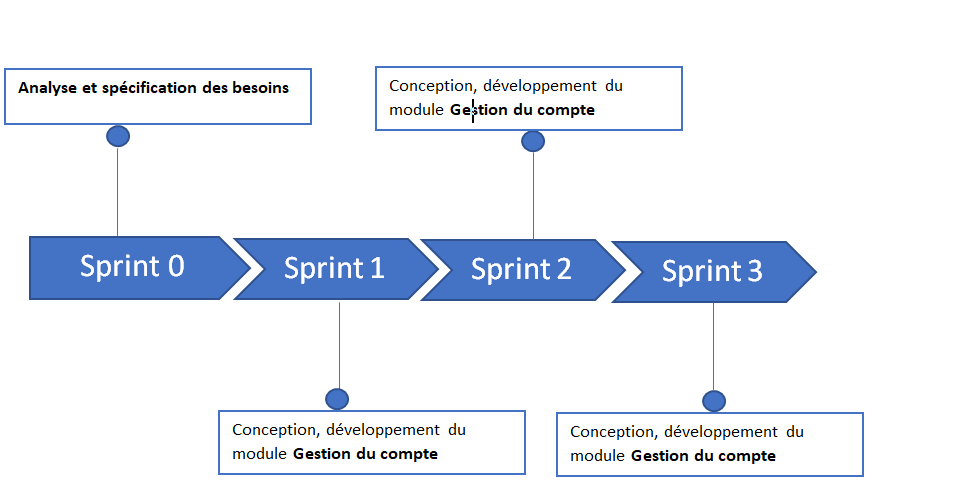
\includegraphics[scale=0.5]{decoupageSprint.PNG}
	\caption{Découpage du projet}
	\label{Découpage du projet}
\end{figure}
\begin{itemize}
	\item \textbf{Sprint 0}: contient une étude préalable du projet.
	\item \textbf{Sprint 1}: \begin{itemize}
		\item Gestion des comptes: contient toutes les fonctionnalités liées à l'accès à l'application et le contrôle des données personnelles.
		\item Gestion des utilisateurs: contient les fonctionnalités liées au contrôle des utilisateurs.

	\end{itemize}  .
\item \textbf{Sprint 2}: 
\begin{itemize}
	\item Management des projets: contient les fonctionnalités liées à la gestion des projets de Tritux.
	\item Management des ressources Cloud: contient les fonctionnalités liées aux contrôle et gestion des ressources Cloud.
\end{itemize}
\item \textbf{Sprint 3}:
\begin{itemize}
	\item Gestion des Planifications.
    \item Gestion des logs

\end{itemize}
\end{itemize}
\subsection{Environnement de travail}
La réussite  de notre travail dépend énormément du choix des technologies et outils utilisés tout en tenant compte du besoin de l'entreprise.
\subsubsection{Choix techniques  pour le Front-end}
\textbf{Angular 7}\\
Angular 7 est la version la plus récente du framework open source Angular, lancé le 18 octobre 2018 par Google. Ce dernier est un framework modulaire à base de components et modules. Il assure 
la création des applications mono-pages (SPA : Signle Page Application), web et mobiles. 
\\ 
Angular 7 propose plusieurs fonctionnalités parmi eux: 
\begin{itemize}
	\item Pipe: Composant permettant la transformation et la personnalisation de l'affichage des données  dans les balises HTML.
	\item Vue: Des fichiers de HTML5 et CSS3.
	\begin{itemize}
		\item  HTML5: Le standard HTML est l'acronyme de « HyperText Mark-Up Language », c'est un
		langage de balisage développé pour la formalisation de l'écriture d'un document. 
		\item CSS3: 
	Les feuilles de styles  sont un langage qui
	permet de gérer la présentation et la mise en forme d'une page web.	
	
	\end{itemize}
	\item Contrôleur: Classe TypeScript représente la logique de la vue. Elle traite les différentes taches à réaliser. Ainsi elle fait le lien entre la vue et les services en invoquant ses méthodes.
	\begin{itemize}
		\item TypeScript: Langage de programmation open-source développé par Microsoft. Il s'agit d'un sur-ensemble syntaxique strict de JavaScript, qui ajoute un typage statique optionnel au langage. TypeScript tend à améliorer et à sécuriser la production du
		code JavaScript.
	\end{itemize}
	\item Services: Composant assurant l'émission, le traitement et la réception des requêtes http, en vue  d'assurer l'échange des données JSON entre les services Web et le contrôleur.
	\begin{itemize}
		\item 
		JSON: JavaScript Object Notation est un format d'échange de données léger. Ainsi, Il est facile pour la lecture et écriture des données. Basé sur le Javascript, le JSON est un format de texte totalement indépendant du langage, c'est-à-dire, il permet de faire communiquer deux langages de programmation différents.
	\end{itemize}
\end{itemize}

\begin{table}[H]  
	

	\begin{tabular}{|l|l|l|l|}
		\hline
		\textbf{Framework}                                                           & \textbf{ReactJS}                                                                                                                             & \textbf{Angular}                                                          & \textbf{Vue}                                                                                                                                  \\ \hline
		\textbf{\begin{tabular}[c]{@{}l@{}}Courbe \\ d'apprentissage\end{tabular}}   & Difficile                                                                                                                                    & Moyen                                                                     & Facile                                                                                                                                        \\ \hline
		\textbf{Scalabilité}                                                         & Haute                                                                                                                                        & Haute                                                                     & Faible                                                                                                                                        \\ \hline
		\textbf{\begin{tabular}[c]{@{}l@{}}Communauté et \\ popularité\end{tabular}} & \begin{tabular}[c]{@{}l@{}}Le plus populaire,\\  entrain de devenir \\ un bon choix pour \\ les applications\\  mobiles natives\end{tabular} & \begin{tabular}[c]{@{}l@{}}Il se développe \\ tellement vite\end{tabular} & \begin{tabular}[c]{@{}l@{}}Une communauté très\\  active et entrain de se\\  développer\end{tabular}                                          \\ \hline
		\textbf{Emplois}                                                             & Fortement demandé                                                                                                                            & \begin{tabular}[c]{@{}l@{}}Fortement\\  demandé\end{tabular}              & \begin{tabular}[c]{@{}l@{}}Moins populaire et \\ n'est pas supporté \\ par une grande \\ entreprise comme \\ Facebook ou Google.\end{tabular} \\ \hline
		\textbf{Performance}                                                         & Haute                                                                                                                                        & moyenne                                                                   & Haute                                                                                                                                         \\ \hline
	\end{tabular}
	\caption{Comparaison des Frameworks les plus populaires du Front-end}
\label{Comparaison des Frameworks les plus populaires du Front-end}
\end{table}
En se basant sur le tableau comparatif 2.2, le choix
du Framework à utiliser a été fixé sur Angular 7 puisqu'il répond parfaitement à nos besoins et aux
exigences techniques du développement de notre application.
\title {Symfony}
\subsubsection{Choix techniques pour le Back-end}
\textbf{Symfony 4} \\
Symfony est un puissant Framework de PHP qui permet de réaliser des sites complexes rapidement, mais de façon structurée et avec un code clair, maintenable et sécurisé en respectant les normes
de programmation. Ainsi Symfony bénéficie d'une richesse des bundles (plugins) développés et permettent de séparer la partie métier de la partie données. Ce dernier est utilisé par Tritux pour la plupart des projets web.\\

\subsubsection{Outils}
\begin{itemize}
\item 	\textbf{Cron job} \newline
	Cron est un utilitaire qui planifie l'exécution automatique d'une commande ou d'un script sur le serveur  à des temps prédéfinis ou après certains intervalles prédéfinis. Un travail cron est la tâche planifiée elle-même. Les tâches Cron peuvent être très utiles pour automatiser des tâches répétitives tels que le contrôle  du budget restant du projet et l'automatisation du fonctionnement des VMs.
	\item \textbf{Node.js} \\Node est une plateforme de développement open source permettant d'exécuter du code JavaScript côté serveur. Node est utile pour développer des applications nécessitant une connexion persistante du navigateur au serveur et exécutant sur un serveur HTTP dédié.
	\begin{figure}[H]
		\centering
		
\includegraphics[scale=0.05]{node.png}
		\caption{Logo Nodejs}
		\label{Logo Nodejs}
	\end{figure} 
\item 
\textbf{Git} \\ Git est un système de contrôle de version distribué gratuit et à source ouverte, conçu pour gérer tout projet, du plus petit au plus grand, avec rapidité et efficacité.
	\begin{figure}[H]
	\centering
	
\includegraphics[scale=0.2]{git.png}
	\caption{Logo Git}
	\label{Logo Git}
\end{figure} 
\item \textbf{Postman} \\ Postman est un puissant client HTTP pour tester les services Web, il facilite le test, le développement et la documentation des API en permettant aux utilisateurs de créer rapidement des requêtes HTTP simples et complexes.
	\begin{figure}[H]
	\centering
	
\includegraphics[scale=0.7]{postman.png}
	\caption{Logo Postman}
	\label{Logo Postman}
\end{figure} 

\end{itemize}

\section{Architecture de l'application}
\subsection{Architecture physique de l'application}
Notre application respecte la logique de l'architecture 3-tiers : nous avons un serveur pour la
Base de données, un serveur Web pour recevoir et émettre les requêtes du client et un serveur client.
	\begin{figure}[h]
	\centering
	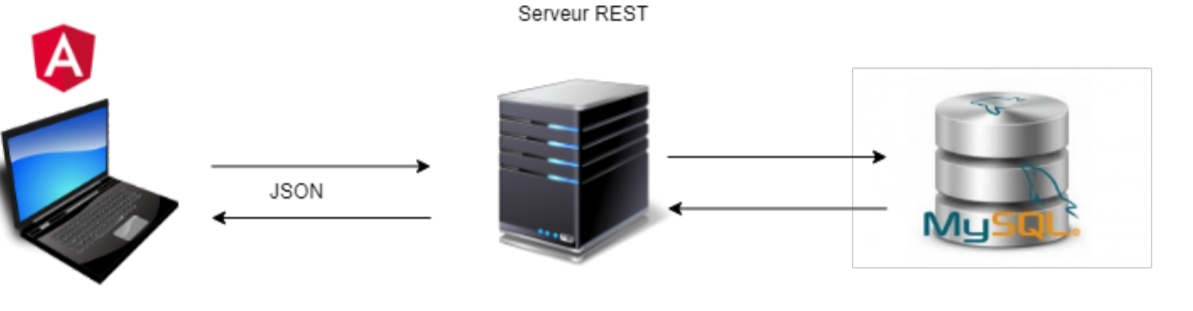
\includegraphics[scale=0.5]{archiphy.PNG}
	\caption{Architecture physique de l'application}
	\label{Architecture physique de l'application}
\end{figure} 
\begin{itemize}
	\item Couche de présentation: Elle correspond à la partie visible et interactive de l'application
	pour les utilisateurs.
	\item Couche de logique métier: Elle permet d'appliquer les règles du métier gérées par
	l'application. Elle agit sur les données capturées à partir de la couche d'accès des données.
	\item Couche d'accès aux données: Elle correspond aux données qui sont destinées à être conservées.
\end{itemize}
La communication entre le client et le serveur REST est assurée par le biais d'échange des APIs REST.
\subsubsection{API REST}
REST est une API qui utilise les méthodes HTTP pour accéder à des ressources
distantes sur le web. Chaque ressource est représentée par une URI 6 qui permet d'avoir
un système universel d'identification des éléments de l'application. Elle supporte plusieurs
formats de données comme JSON, XML, YML.
\subsection {Architecture logique de l'application}

\subsubsection{Architecture Front-end}


	\begin{figure}[h]
	\centering
	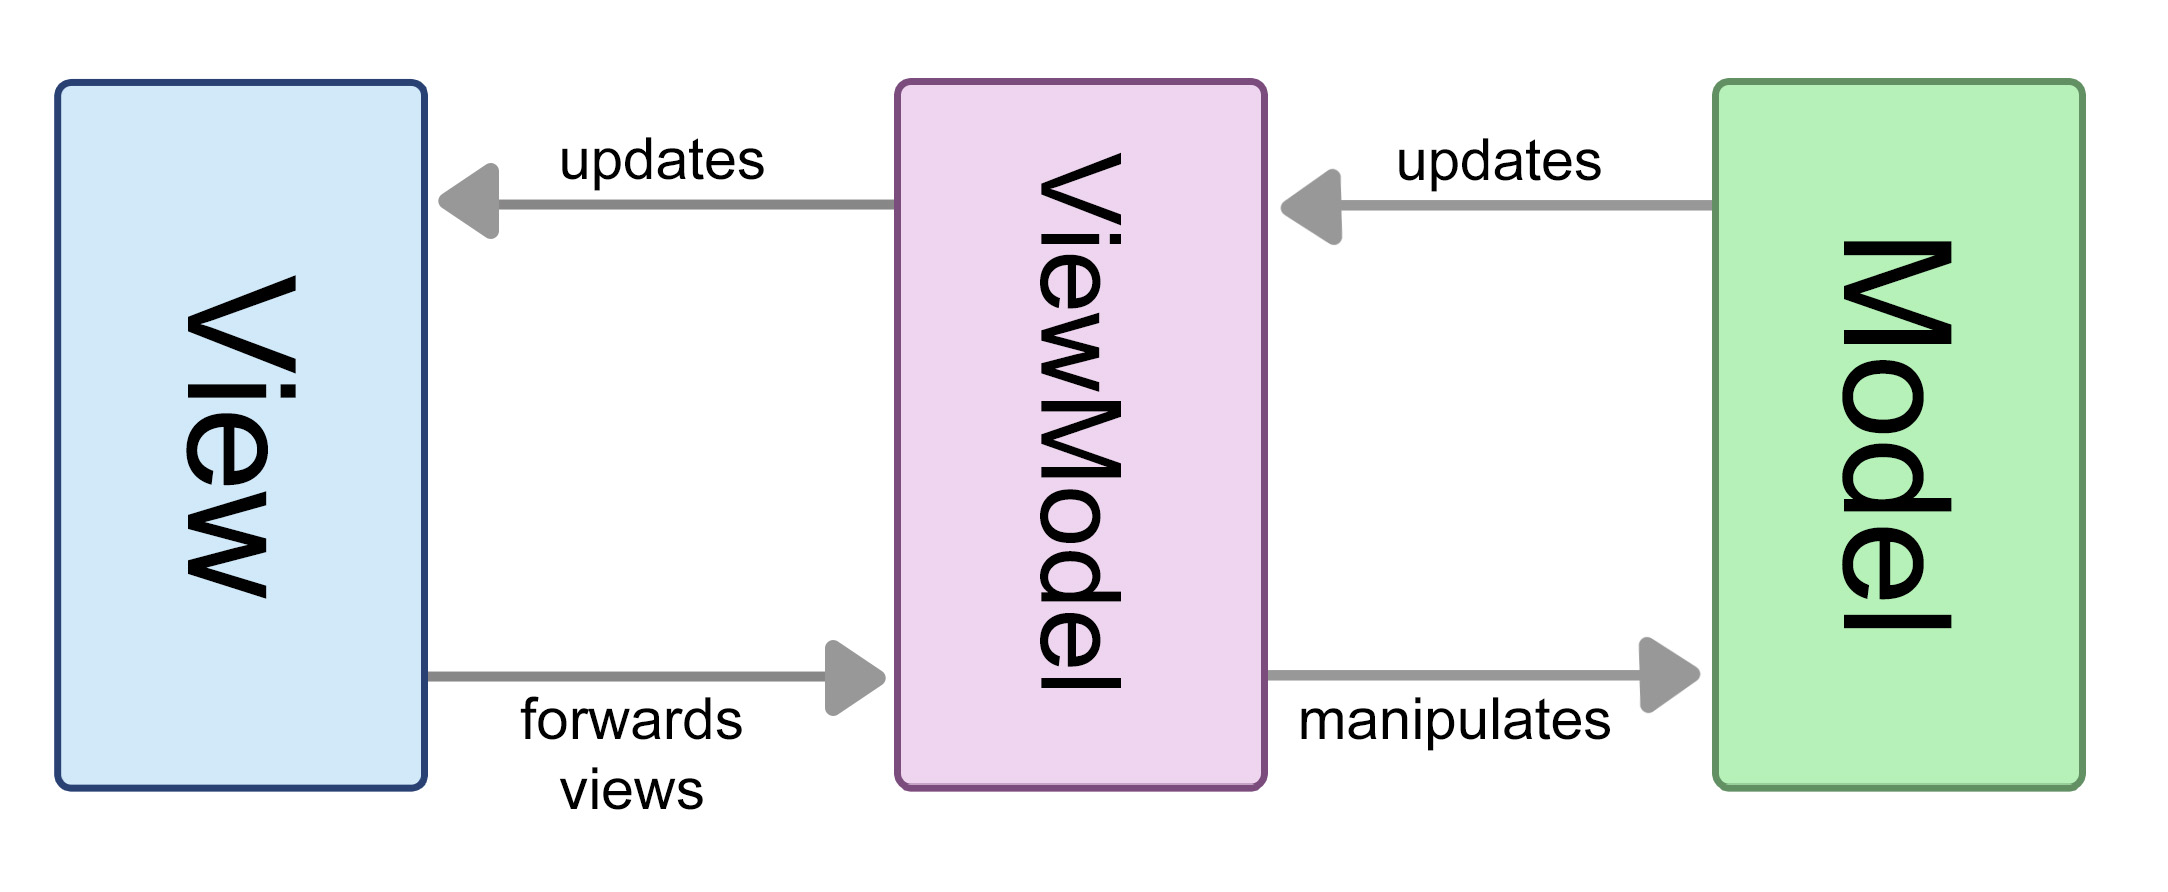
\includegraphics[scale=0.1]{mvvm.jpg}
	\caption{Architecture logique Front-end de l'application}
	\label{Architecture logique Front-end de l'application}
\end{figure} 
MVVM pour model view view-Model est un design pattern qui facilite la séparation du développement de l'interface utilisateur, c'est-à-dire de la couche de présentation.\\Comme le montre la figure 2.12  ViewModel (VM) est chargé d'exposer les objets de données du modèle de manière à ce que les objets soient plus facilement gérés et présentés.\\
Pour son architecture, Angular adopte le modèle MVVM, cette implémentation est présentée comme suit : 
%il faut verifier l'architecture logique d'angular
\begin{itemize}
	\item \textit{Model}  est implémenté en tant que service angulaire.
	\item \textit{View}  est implémentée à l'aide d'un modèle angulaire.
	\item \textit {ViewModel}  est implémenté en tant que contrôleur angulaire. La directive 'ngController' permet de spécifier un contrôleur pour une vue.
\end{itemize}
\subsubsection{Architecture Back-end}

Symfony est basée sur l'architecture MVC (modèle, vue et contrôleur) qui est  
un modèle architectural très puissant, il
tire sa puissance de son concept de base qui est la séparation des données (modèle), de
l'affichage (vue) et des actions (contrôleur).
	\begin{figure}[H]
	\centering
	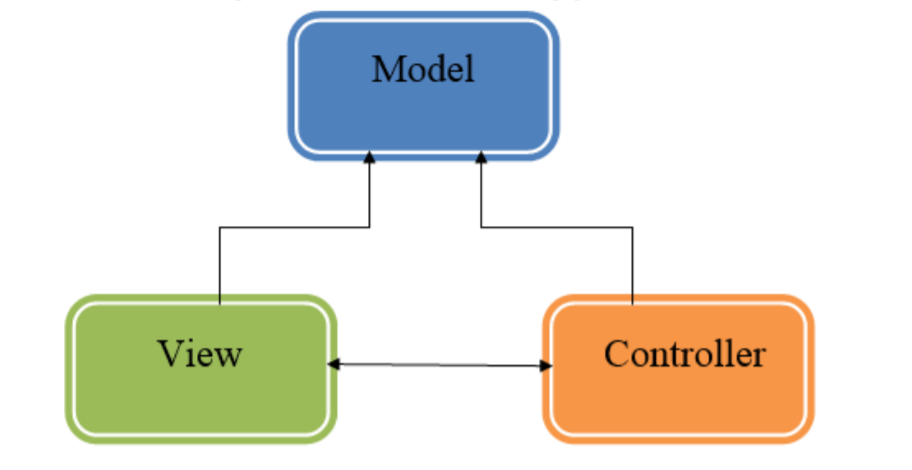
\includegraphics[scale=0.5]{archisym.PNG}
	\caption{Architecture logique Back-end de l'application}
	\label{Architecture logique Back-end de l'application}
\end{figure} 

\section{Conclusion}
Ce chapitre nous a été utile pour montrer notre objectif, nos besoins et éclaircir notre
démarche à travers l'identification des acteurs et des besoins. Il nous a offert une vision plus détaillée en réalisant  une étude conceptuelle globale et en présentant les spécificités techniques de l'application. Le chapitre suivant sera consacré à réaliser le premier incrément de notre projet.